\documentclass[]{notex}
\usepackage{notexmacros}

\usepackage{blindtext}
\usepackage{makecell}
\usepackage{tikz}

\newtcolorbox{doccommand}[1]{
    colback = maindoccol
}
\newcommand{\becomes}[1]{\hspace{#1} $\--$becomes$\rightarrow$ \hspace{#1}}
\newcommand{\littlebox}[1]{\begin{tikzpicture}
    \fill[#1, very thick] (0, 0) rectangle (1, 0.5);
\end{tikzpicture}}

\title{NoTeX}
\author{ElBi21 - Leonardo Biason}
\date{Somewhere in 2024}

\begin{document}

%\maketitle
\begin{titlepage}
    \begin{center}
        \titleheader
        \vspace{0.75cm}

        \hrule
        \vspace{2cm}
        {\huge \textbf{\textsc{\titlecourse}}}
        \linebreak
        
        \vspace{1.5cm}
        \begin{tikzpicture}
            \begin{scope}
                \clip [rounded corners=.5cm] (0, 0) rectangle coordinate (centerpoint) (15, 7.5cm); 
                \node [inner sep=0pt] at (centerpoint) {\includegraphics[width=\linewidth]{\titlecover}}; 
            \end{scope}
        \end{tikzpicture}
        \vspace{2.5cm}

        \hrule
        
        \vspace{1.5cm}
        {\Large \textsc{Notes by \titleauthor}}
        \linebreak
        {\large \textsc{\titlesubtitle}}
        \linebreak
        
        \vspace{2cm}
        \titlefooter
    \end{center}
\end{titlepage}

\chapter{Introduction}

\noindent This is an attempt to transform the old project of NoTeX into an actual class, done in a proper way. The class is based out of the \texttt{report} class, and all the parameters are defined in the \texttt{notex.cls} class file. The class comes with a packet, called \texttt{notexmacros}. Such packet adds plenty of macros that can be used by the user, and that were pretty much useful to me while taking notes. This class aims also to reduce drastically the number of errors and thus increase the compile time. If it will be worth, it will be published also on the \texttt{CTAN} archive.

\chapter{The \texttt{notex} class}

The class file is organized in various structures: \textbf{declaration}, \textbf{packages importation}, \textbf{definition of colors}, \textbf{custom commands}, \textbf{loading of the class}.

\section{Declaration}

The declaration of the class simply consists of the following lines of command:
\begin{tcolorbox}
    \begin{verbatim}
\NeedsTeXFormat{LaTeX2e}
\ProvidesClass{notex}[2024 ElBi21 LaTeX class for taking notes]\end{verbatim}
\end{tcolorbox}

\section{Importing the packages needed}

The following packages are imported into the \texttt{notex.cls} class file:
\begin{tcolorbox}
    \begin{verbatim}
\RequirePackage{xcolor}                 % Package for colors
\RequirePackage{tcolorbox}              % Package for boxes
\RequirePackage[a4paper]{geometry}      % Package for the geometry of the file
\RequirePackage{listings}               % Package for code

\RequirePackage[T1]{fontenc}            % Package for font encoding
\RequirePackage{fouriernc}              % Package with the font
\RequirePackage{sourcecodepro}

\RequirePackage{notexmacros}            % Package with macros
    \end{verbatim}
\end{tcolorbox}

\pagebreak
\section{Custom colors}

There are some colors that are added from the class. This list reports all of them, alongside a quick preview:

\begin{center}
    \begin{tabular}{c l}
        \textbf{Color Preview} & \textbf{Name of the color} \\
        \hline
        \littlebox{maindoccol} & \makecell[l]{\texttt{maindoccol}} \\
        \hline
        \littlebox{theoryLINE} & \makecell[l]{\texttt{theoryLINE}} \\
        \littlebox{practiceLINE} & \makecell[l]{\texttt{practiceLINE}} \\
        \littlebox{curiosityLINE} & \makecell[l]{\texttt{curiosityLINE}} \\
        \littlebox{remarkLINE} & \makecell[l]{\texttt{remarkLINE}} \\
        \hline
        \littlebox{lemmaBG} & \makecell[l]{\texttt{lemmaBG}} \\
        \littlebox{lemmaTitleBG} & \makecell[l]{\texttt{lemmaTitleBG}} \\
        \littlebox{definitionBG} & \makecell[l]{\texttt{definitionBG}} \\
        \littlebox{definitionTitleBG} & \makecell[l]{\texttt{definitionTitleBG}} \\
        \littlebox{corollaryBG} & \makecell[l]{\texttt{corollaryBG}} \\
        \littlebox{corollaryTitleBG} & \makecell[l]{\texttt{corollaryTitleBG}} \\
        \littlebox{proofBG} & \makecell[l]{\texttt{proofBG}} \\
    \end{tabular}
    \begin{tabular}{c l}
        \textbf{Color Preview} & \textbf{Name of the color} \\
        \hline
        \littlebox{theoremBG} & \makecell[l]{\texttt{theoremBG}} \\
        \littlebox{theoremTitleBG} & \makecell[l]{\texttt{theoremTitleBG}} \\
        \littlebox{exerciseBG} & \makecell[l]{\texttt{exerciseBG}} \\
        \littlebox{exerciseTitleBG} & \makecell[l]{\texttt{exerciseTitleBG}} \\
        \littlebox{exampleBG} & \makecell[l]{\texttt{exampleBG}} \\
        \littlebox{exampleTitleBG} & \makecell[l]{\texttt{exampleTitleBG}} \\
        \littlebox{solutionBG} & \makecell[l]{\texttt{solutionBG}} \\
        \littlebox{solutionTitleBG} & \makecell[l]{\texttt{solutionTitleBG}} \\
        \hline
        \littlebox{remarkBG} & \makecell[l]{\texttt{remarkBG}} \\
        \littlebox{remarkTitleBG} & \makecell[l]{\texttt{remarkTitleBG}} \\
        \hline
        \littlebox{curiosityBG} & \makecell[l]{\texttt{curiosityBG}} \\
        \littlebox{curiosityTitleBG} & \makecell[l]{\texttt{curiosityTitleBG}} \\
        % Space adder
        %\littlebox{white} & \\
    \end{tabular}
\end{center}

\section{Commands of the class}

This class provides various commands, which allow to customize to your liking the template. Here is a list of all the supported (and provided) commands:

\begin{tcolorbox}
    \verb|\maincol{format}{code}|
    \tcblower
    \begin{tabular}{r l}
        \textbf{Examples}: & \verb|\maincol{HTML}{303342}| \\ 
                           & \verb|\maincol{RGB}{30, 25, 76}|
    \end{tabular}
\end{tcolorbox}

\noindent Sets the main color for the document.
\begin{itemize}
    \item [\texttt{format}] specifies the format of the color. Supports all the formats of the \texttt{xcolor} package;
    \item [\texttt{code}] is the code of the color. Must match the format given by the previous parameter
\end{itemize}

\section{Loading of the class}

\section{Custom boxes}

The NoTeX class adds also some custom boxes, which are helpful when there is the need to mark some important parts of the text, such as definitions, theorems, proofs, code, etc... Here is a showcase of all the boxes and how they can interact with each other.

\begin{definition}{Uniform Resource Identifier (URI)}
    A \textbf{Uniform Resource Identifier} (\textbf{URI} for short) is a unique sequence of characters which identifies a logical or physical resource. An example of URI might be:
    
    \medskip

    \texttt{https://thisisanexample.com/usernames}
\end{definition}

\begin{theorem}{Spectral Theorem}
    Given a matrix $A$ which is \textbf{squared} ($A \in \mathbb{R}^{d \times d}$) and \textbf{symmetric} ($A \eq A^\top$), then \textbf{all the eigenvalues} $\lambda_i$ take \textbf{real values} and \textbf{all the eigenvectors} are \textbf{orthogonal}
    
    \begin{proof}
        This can be easily proved as follows:\\
        \noindent The $\nabla$ is equal to 1\\
        \noindent The matrices are equal
    \end{proof}
\end{theorem}

\begin{lemma}{Running time of the algorithm}
    If the algorithm receives as an input an ordered list of items, then its running time will be at most $O(n)$. If the list isn't ordered, then it will take at most $O(n \log(n))$

    \begin{proof}
        In order to prove this algorithm, we must first consider the running time of the sub-algorithm. Indeed, we'll obtain that:
        \[ \text{runtime} \eq O(n \log(n)) + O(n) \]
    \end{proof}
\end{lemma}

\begin{corollary}{Sum of internal angles of triangles}
    Given any triangle, the sum of its internal angles will always be equal to $180\degree$. Moreover, if the triangle is equilateral, then all its angles will be equal to $60\degree$
\end{corollary}
\medskip
\noindent The \textbf{definition}, \textbf{theorem}, \textbf{lemma} and \textbf{corollary} boxes can be called with:
\begin{tcolorbox}
    \begin{verbatim}
\begin{<box_type>}{<term>}
    Your text...
\end{<box_type>}\end{verbatim}

\noindent where \verb|<box_type>| can be one between \texttt{definition}, \texttt{theorem}, \texttt{lemma} and \texttt{corollary}, while instead \verb|<term>| denotes the title of the box
\end{tcolorbox}

\noindent It is instead possible to invoke the \textbf{proof} box by using the following command:

\begin{tcolorbox}
    \begin{verbatim}
\begin{proof}
    Your proof...
\end{proof}\end{verbatim}
\end{tcolorbox}

\noindent The proof box can be used anywhere, it is however thought for the \textbf{theorem} and \textbf{lemma} boxes (since definitions and corollary should not need proofs).

\begin{exercise}
    Solve the following equation:
    \[ x^2 + \sin(3x-4) - 7 \eq 6 \]
\end{exercise}

\begin{example}
    An example of limit is the following:
    \[ \lim_{x \to 0} \log_{10}(x+1) \eq +\infty \]
\end{example}

\pagebreak

\begin{codeblock}{TestCode.py}
    \begin{lstlisting}[language = Python]
def main():
    for i in range(40):
        print(i)
    return None\end{lstlisting}
\end{codeblock}

\begin{terminal}
    \begin{lstlisting}[style = notexterm]
$ mpicc 01-mpi-collectives.c -o 01-mpi-collectives.o\end{lstlisting}
\end{terminal}

\chapter{The title page}

NoTeX also offers the possibility of having a custom title page. Clearly, you are free to edit it to your liking. The template comes with some pre-defined values, and has the following structure:

\begin{center}
    \begin{tikzpicture}
        \node [inner sep=0pt] at (centerpoint) {
            \setlength{\fboxsep}{0pt}
            \setlength{\fboxrule}{0.5pt}
            \fbox{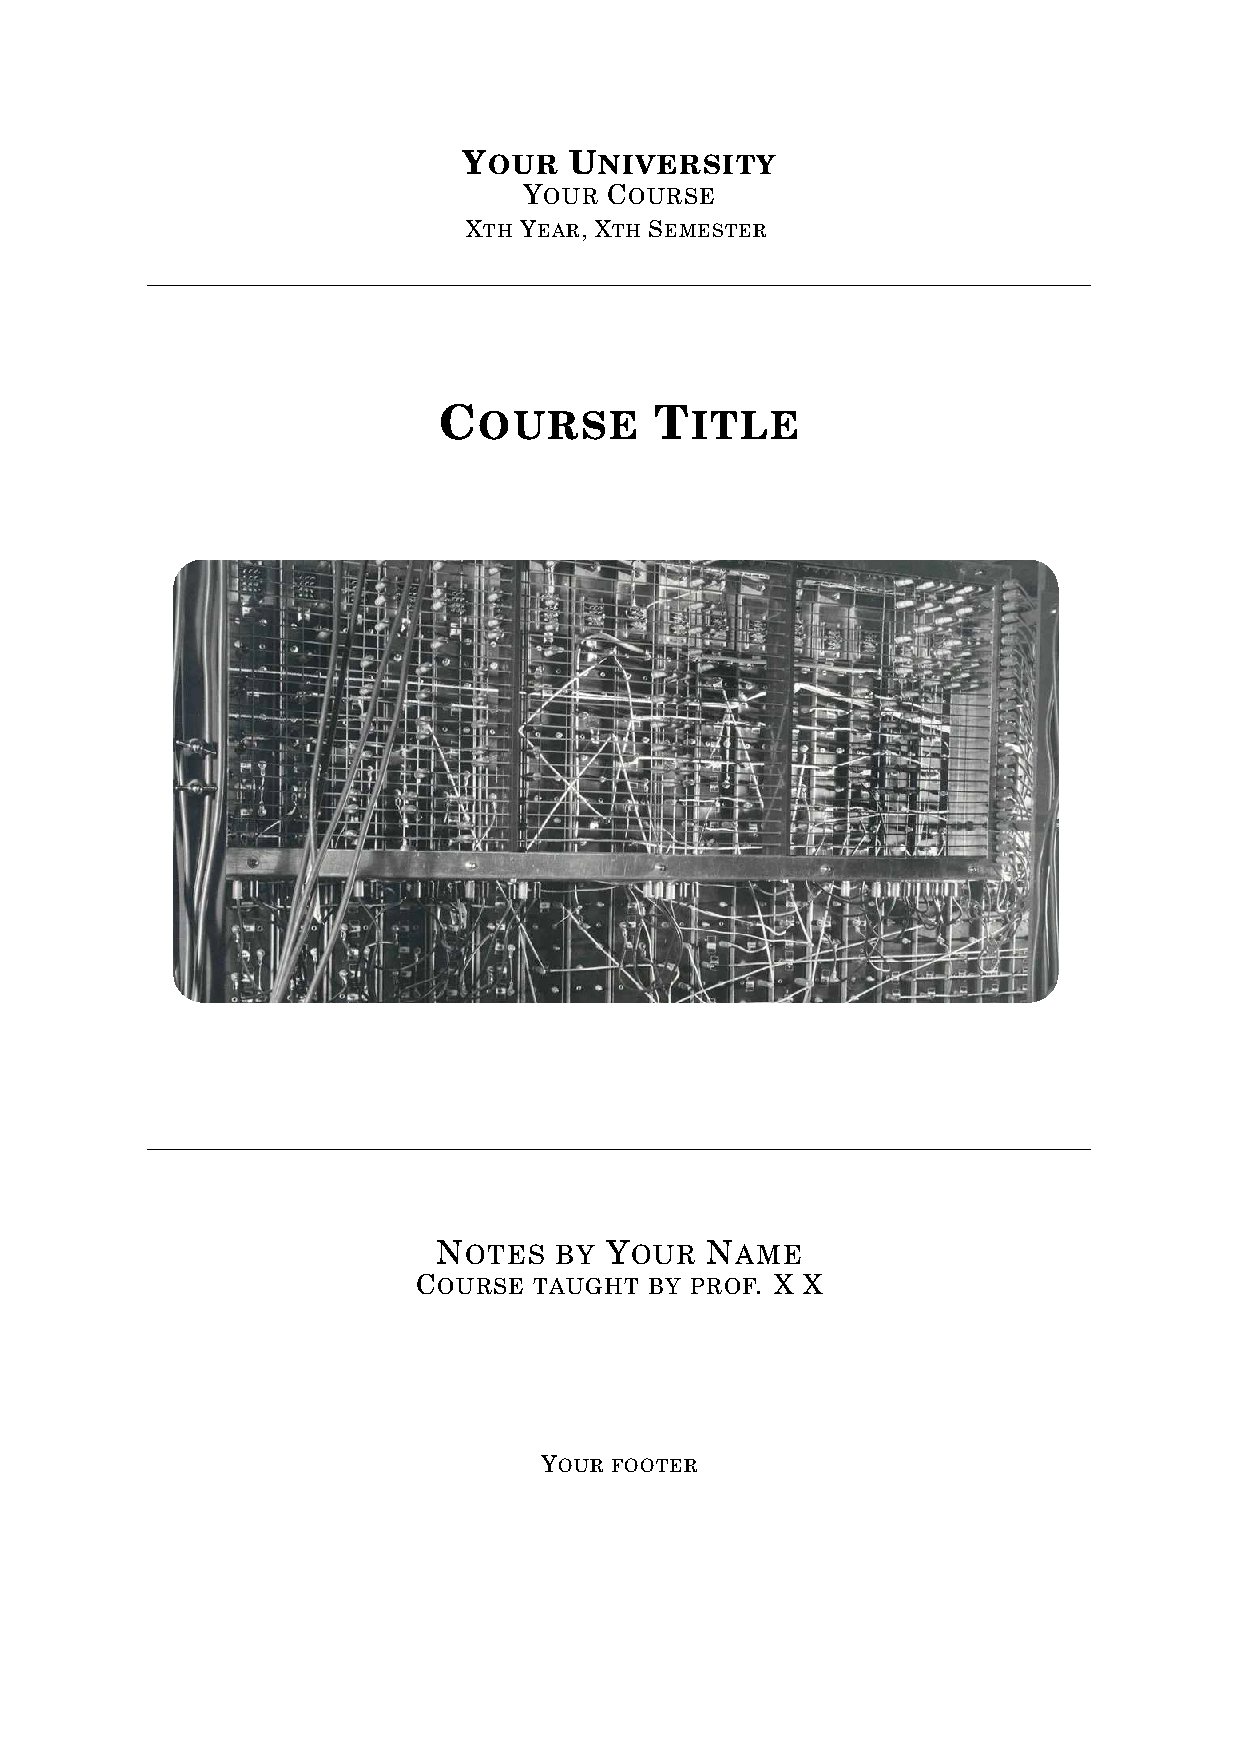
\includegraphics[width=0.5\linewidth]{assets/title-page.pdf}}
        };
        \draw[red!60, thick, <-] (6.25, 8.15) -- (2.5, 8.15) node[anchor=east]{Header};
        \draw[red!60, thick, <-] (4.5, 4.5) -- (2.5, 4.5) node[anchor=east]{Cover};
        \draw[red!60, thick, <-] (6, 1.14) -- (2.5, 1.14) node[anchor=east]{Subtitle};

        \draw[red!60, thick, <-] (9, 6.65) -- (12.75, 6.65) node[anchor=west]{Title};
        \draw[red!60, thick, <-] (9, 1.35) -- (12.75, 1.35) node[anchor=west]{Author};
        \draw[red!60, thick, <-] (8.5, -0.05) -- (12.75, -0.05) node[anchor=west]{Footer};
    \end{tikzpicture}
\end{center}

You can edit the following parts by renewing the commands with the \verb|\renewcommand| command:
\begin{itemize}
    \item \textbf{header}: renew \verb|\titleheader| with what you want to put into the header. You can put anything you'd like, images included;
    \item \textbf{title}: renew \verb|\titlecourse| with the name of the course that would go on the title. Only text is allowed, any other item will result in unknown behaviour;
    \item \textbf{cover}: renew \verb|\titlecover| with the path of the image you want to replace. Only paths are allowed, any other item will result in unknown behaviour;
    \item \textbf{author}: renew \verb|\titleauthor| with your name. Only text is allowed, any other item will result in unknown behaviour;
    \item \textbf{subtitle}: renew \verb|\titlesubtitle| with the subtitle that you desire. Only text is allowed, any other item will result in unknown behaviour;
    \item \textbf{footer}: renew \verb|\titlefooter| with anything you want to put into the footer. You can put anything you'd like, images included.
\end{itemize}

If you don't like the title page, you are free to edit it or to add your own version. If you want a more "classic" title page, you can use the \verb|\title|, \verb|\author| and all the other standard commands provided by \LaTeX.

\chapter{The \texttt{notexmacros} package}

\noindent In this chapter the \texttt{notexmacro} package will be explained. Such package contains a collection of macros which can turn to be useful while using the class. The package is automatically required by the class, so you don't have to install anything else.
\\
\indent The macros are divided into two groups: the \textbf{math} macros and the \textbf{text} macros. The \textbf{math} macros are used within a math environment, while the text macros are not. There are some \textbf{general purpose} macros which can be used both inside and outside a \textbf{math} environment.

\section{The \texttt{math} macros}

\begin{tcolorbox}
    \verb|\eq|
\end{tcolorbox}

\noindent Adds space around a $=$. An example follows:
\begin{center}
    \verb|a \eq b| \becomes{20pt} $a \eq b$
\end{center}

\begin{tcolorbox}
    \verb|\thus|
\end{tcolorbox}

\noindent Adds substantial space around a $\Longrightarrow$, and it can be used to define a logical implication (\textit{we have $A$, thus we can get $B$}). An example follows:
\begin{center}
    \verb|a \thus b| \becomes{20pt} $a \thus b$
\end{center}

\begin{tcolorbox}
    \verb|\nextline| and \verb|\prevline|
\end{tcolorbox}

\noindent Adds a $\Longrightarrow$ which can be used at the end (with \verb|\nextline|) or at the beginning (with \verb|\prevline|) of an equation. This can be used while passing from one line to the other of an equation which would usually need more than one line. An example follows:
\begin{center}
    \verb|ax + b \nextline| \becomes{20pt} $ax + b \nextline$ \\
    \verb|\prevline ax + c| \becomes{20pt} $\prevline ax + c$
\end{center}

\subsection{Specific macros for statistical distributions}

\begin{tcolorbox}
    \verb|\cov|, \verb|\bino|, \verb|\berno|, \verb|\unif|, \verb|\geom|, \verb|\poiss| and \verb|\multin|
\end{tcolorbox}

\noindent Adds the function of the covariance and the following distributions: the binomial distribution, the Bernoulli distribution, the uniform distribution, the geometric distribution, the Poisson distribution and the multinomial distribution. An example follows:
\begin{center}
    \begin{tabular}{c c c}
        \verb|\cov(X)| & \becomes{20pt} & $\cov(X)$ \\ & & \\
        \verb|X \sim \bino \sim \berno \sim \unif| & \becomes{20pt} & $X \sim \bino \sim \berno \sim \unif$ \\
        \verb|\sim \geom \sim \poiss \sim \multin| & & $\sim \geom \sim \poiss \sim \multin$
    \end{tabular}
\end{center}

\section{The \texttt{text} macros}

\begin{tcolorbox}
    \verb|\angbrack{}|
\end{tcolorbox}

\noindent Wraps the content between two angle brackets. Works both in a \texttt{math} and in a non-\texttt{math} environment. An example follows:
\begin{center}
    \verb|\angbrack{10}| \becomes{20pt} \angbrack{10}
\end{center}

\begin{tcolorbox}
    \verb|\st|, \verb|\nd|, \verb|\rd| and \verb|\nth|
\end{tcolorbox}

\noindent Adds respectively the \textit{st}, the \textit{nd}, the \textit{rd} and the \textit{th} after a number. Works both in a \texttt{math} and in a non-\texttt{math} environment. An example follows:
\begin{center}
    \verb|1\st, 2\nd, 3\rd, 4\nth| \becomes{20pt} 1\st, 2\nd, 3\rd, 4\nth
\end{center}

\end{document}